\section{Linear Filtering}

Filtering an image is a way to augment or extract information from it. Linear filters are a subset of operations that operate on a neighbourhood of pixels in an image. A filter's size determines the size of the neighbourhood to take as input for the operation. All linear filters operate on the same prinicpal, that is, they output a weighted average of their input. It is the weightings of a filter, known as filter coefficients, that determine the effect of the filter. These weights are stored in a matrix called a mask or kernel (see Figure \ref{fig:generalForm}) that's then convolved or correlated with an image.

\begin{figure}[h]
  
   \[ 
     Kernel  = \frac{1}{\sum\limits_{i=0}^{M}\sum\limits_{j=0}^{N}c_{i,j}}
    \begin{bmatrix}
      c_{0,0} & c_{0,1} & \dots & c_{0,n} \\
      c_{1,0} & c_{1,1} & \dots & c_{1,n} \\
      \vdots & \vdots & \ddots & \vdots \\
      c_{m,0} & c_{m,1} & \dots & c_{m,n}
    \end{bmatrix}
  \]
  \caption{General Form of a Linear Filter}
  \label{fig:generalForm}
\end{figure}

 A filter kernel is nearly always square so as to have a center cell which sits atop a reference pixel. The result of the filter's application at that reference pixel will be stored in the output image at the location of the reference pixel. Notice in Figure \ref{fig:kernel_graphics} how the mask sits over the reference pixel.

% TREE %
\begin{figure}[H]
  \centering
  \centering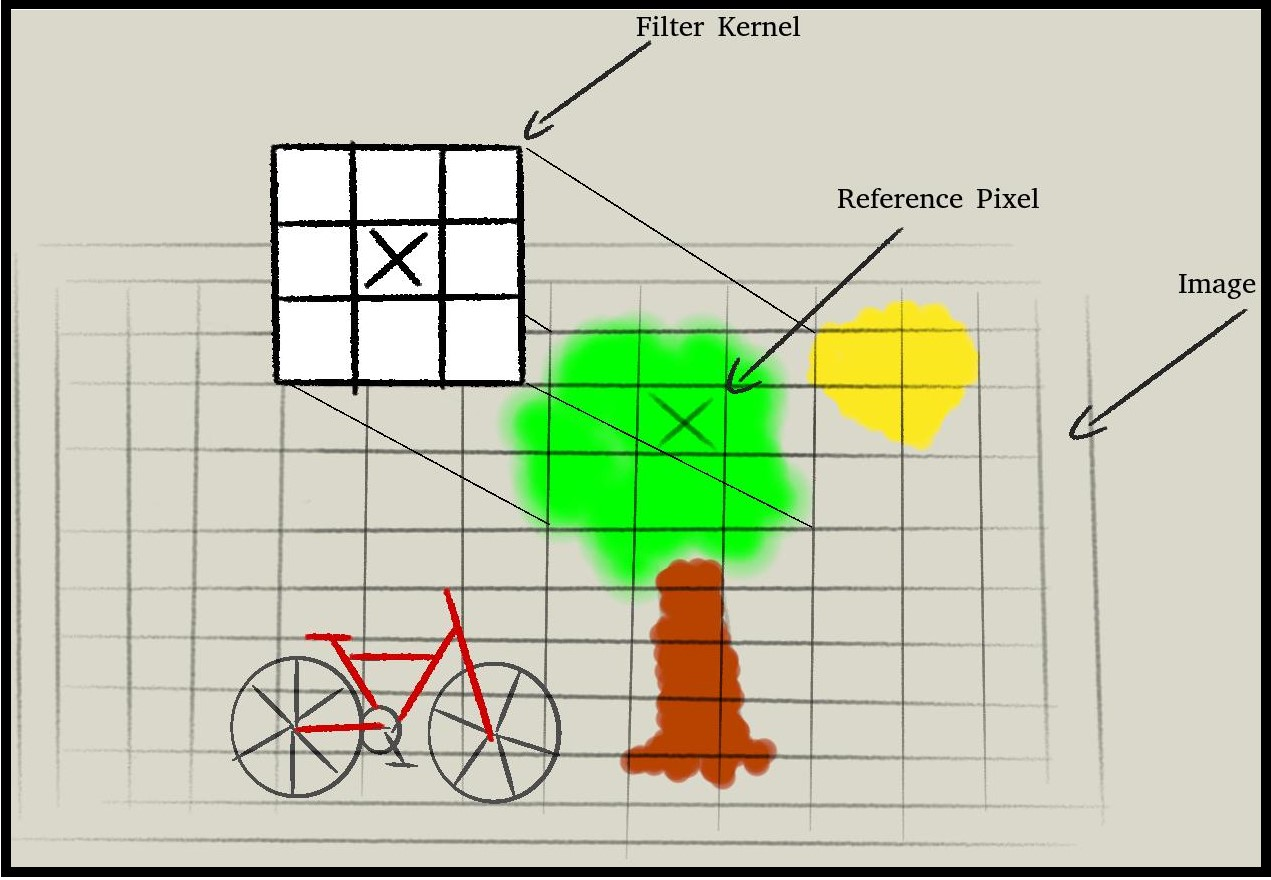
\includegraphics[width=350pt]{kernel_graphics}
  \caption{Visualization of a Filter Kernel Application}
  \label{fig:kernel_graphics}
\end{figure}

A 'box filter', for example, outputs the average of its inputs. This is because the filter weights are evenly distributed. By passing this filter over an image its sharpness is reduced giving a smoothing or blurring effect. This can be observed in Figure \ref{fig:roughDog}.

% DOG %
\begin{figure}[H]
  \centering
  \centering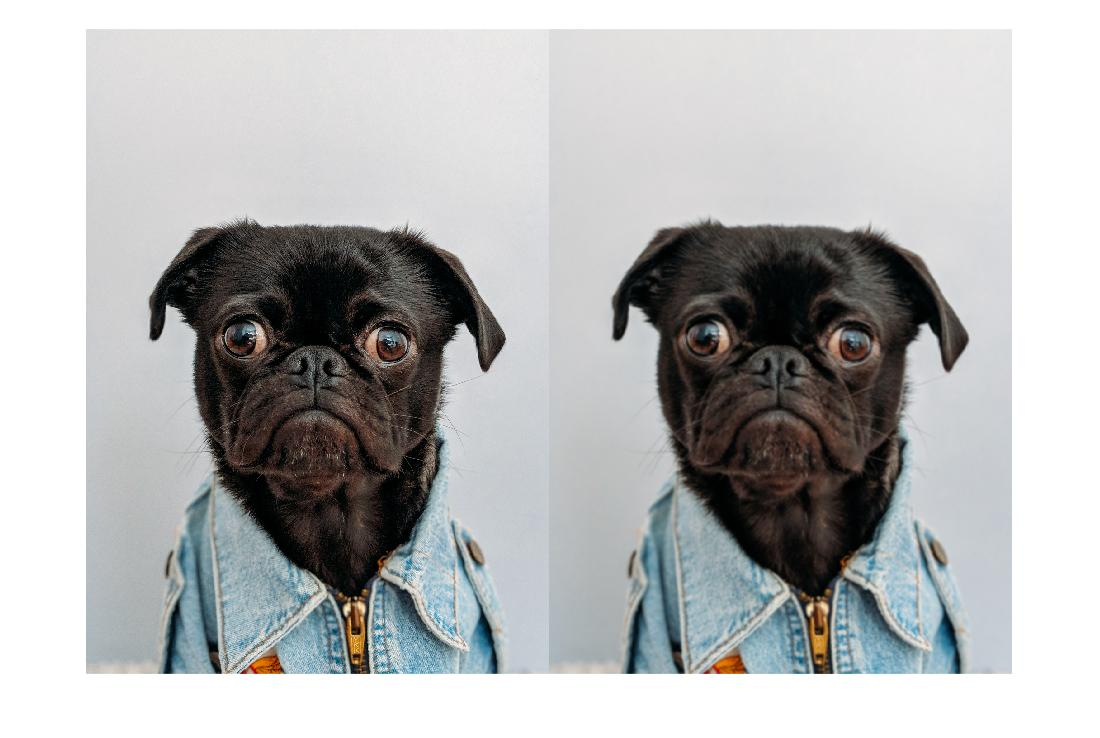
\includegraphics[width=350pt]{dogPug}
  \caption{Left image is the original and the right image has had $16\times16$ box filter applied. \emph{Photo by Charles Deluvio on Unsplash.}}
  \label{fig:roughDog}
\end{figure}

\subsection{Correlation}

The application of a linear filter $h(u,v)$ to an image $f(i,j)$ may be described as follows

\begin{equation} \label{eq:1}
g(i,j) = \sum_{u=-k}^{k}\sum_{v = -l}^{l}f(i+u,j+v)h(u,v)
\end{equation}


The dimensions of the filter kernel are ($2k+1) \times (2l+1$). Filter kernels are nearly always odd dimensioned so as to have a center. This is because an asymmetric kernel, one which has even numbered dimensions, will result in output being distorted. This is because the output from the filter will be weighted unevenly by being placed in a reference pixel that is not centered causing aliasing.

\begin{figure}[H]
  \centering
  \centering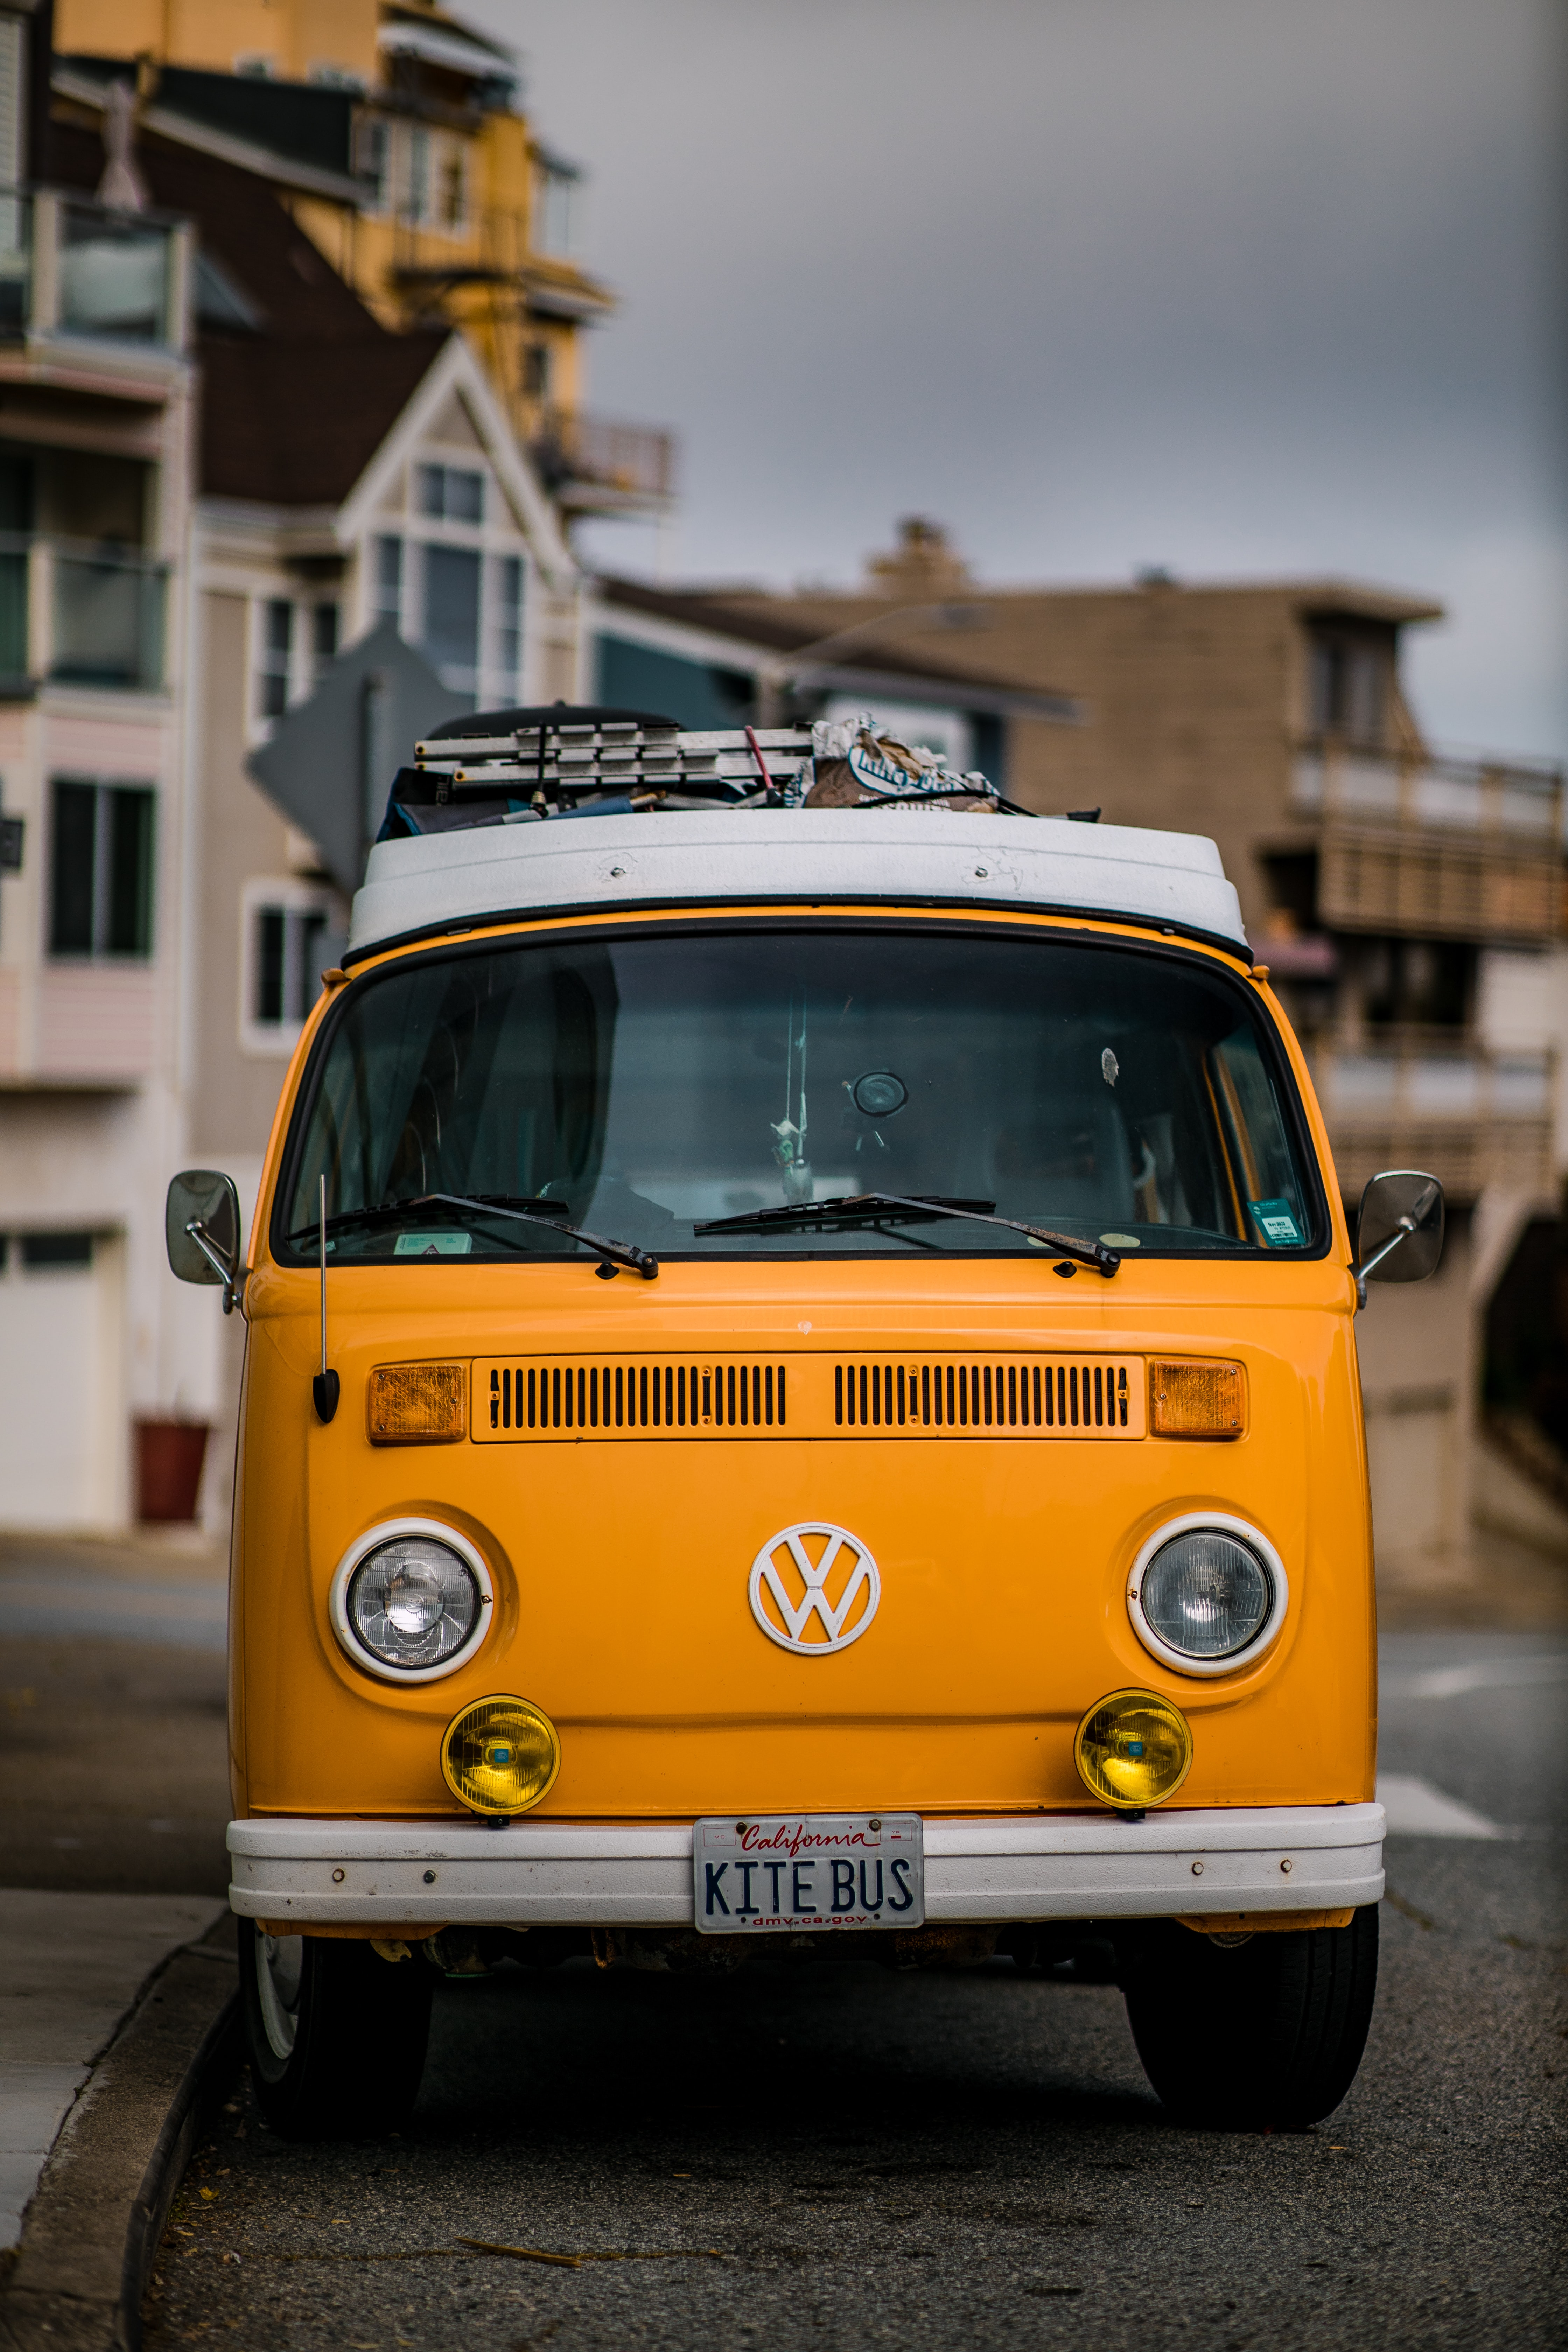
\includegraphics[width=200pt]{van}
  \caption{SHOW IMAGE ALIASING. Photo by Jason Leung on Unsplash}
  \label{fig:van}
\end{figure}

Performing correlation with a filter may be notated more concisely by the \emph{correlation} operator.

\[g = f \otimes h\]

Correlation measures the similarity between two signals. Both digital images and linear filters are two dimensional signals. Performing correlation between them will yield an image where the highest values output correspond to where the image and filter are most similar \cite{optimalKernel}. This useful because if you wish to emphasise a feature in an image it can be done by correlating a filter that describes that feature with an image. For example, if you wished to exagerate straight vertical lines you would apply a filter that looks like a straight vertical line,

\[ 
\begin{bmatrix}
  0 & 1 & 0 \\
  0 & 1 & 0 \\
  0 & 1 & 0
\end{bmatrix}
\]


\begin{figure}[htbp]
  \centering
  \begin{subfigure}[b]{0.3\textwidth}
      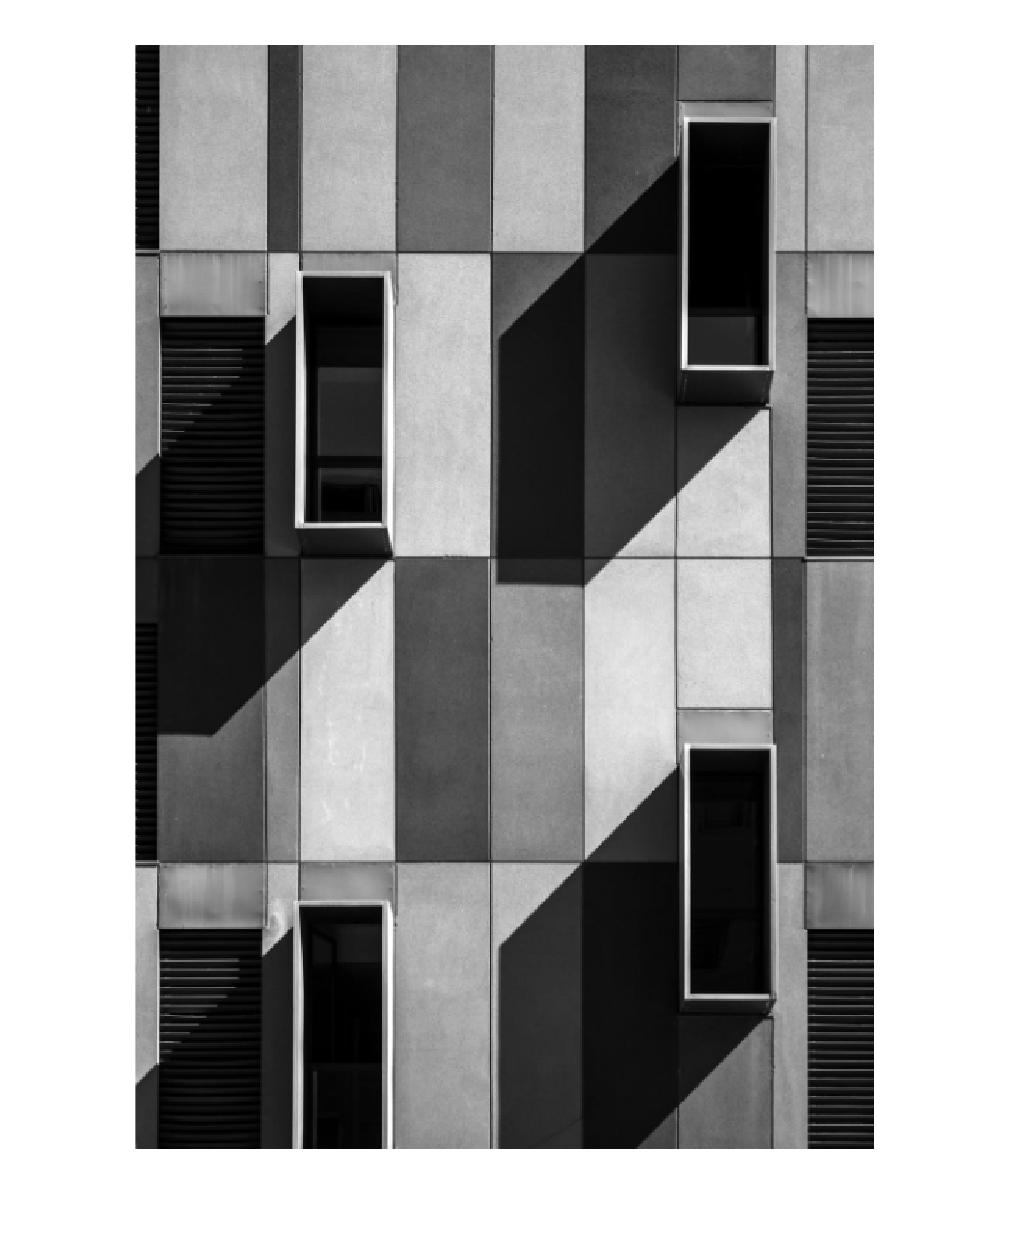
\includegraphics[width=\textwidth]{im}
      \caption{Image by Simone Hutsch}
      \label{rfidtest_xaxis}
  \end{subfigure}
  \begin{subfigure}[b]{0.3\textwidth}
      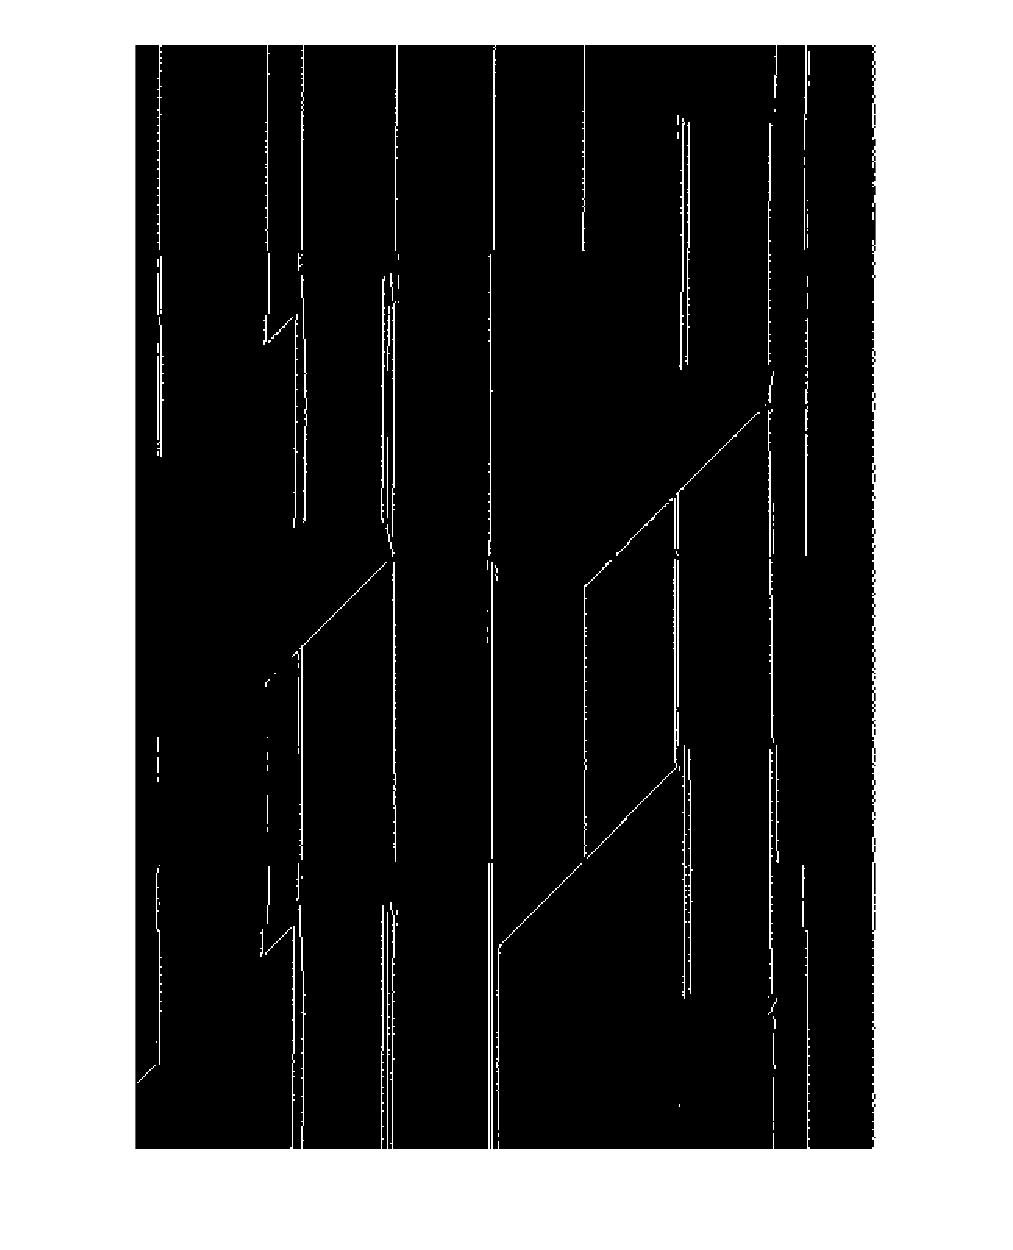
\includegraphics[width=\textwidth]{gv}
      \caption{Vertical Sobel Filter}
      \label{rfidtest_yaxis}
  \end{subfigure}
  \begin{subfigure}[b]{0.3\textwidth}
      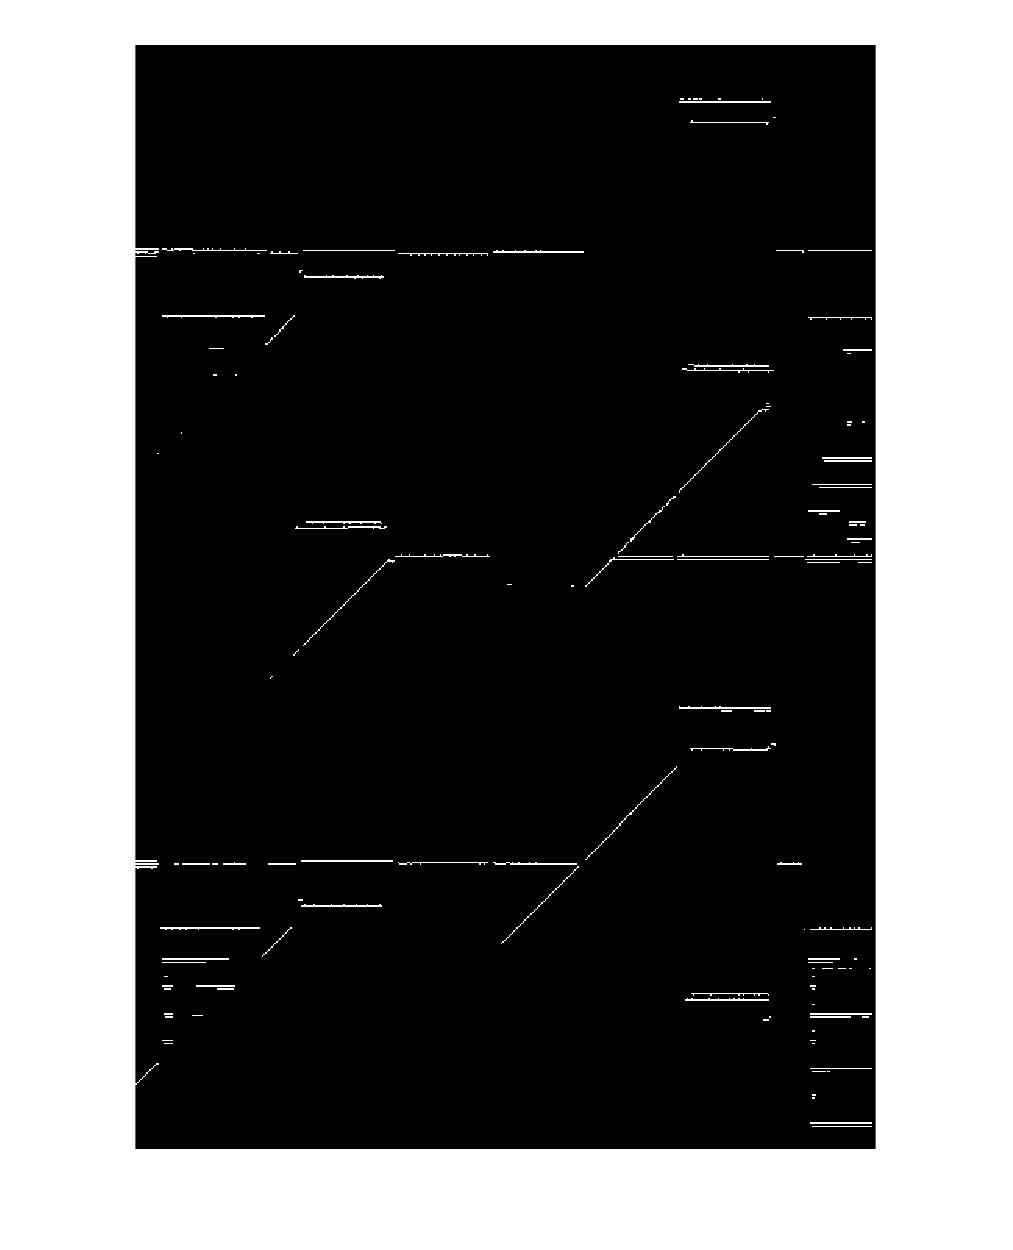
\includegraphics[width=\textwidth]{gh}
      \caption{Horizontal Sobel Filter}
      \label{rfidtest_zaxis}
  \end{subfigure}
  \caption[RFID tag read-range testing]{RFID tag read-range testing setup. In all tests, the finger moves towards along an axis towards the tag.}
  \label{rfidtag_testing}
\end{figure}

This operation is \emph{shift invariant}, which means that it does the same thing no matter where in an image it is applied. Therefore, correlation operations obey both the superposition principle

\[a(f_1 + f_2) = af_1 + af_2\]

and the shift invariance principle

\[g(i,j)=f(i+k,j+l) \Leftrightarrow\ (h\circ g)(i,j)=(h\circ f)(i+k,j+l)\]

This operation has the side effect of flipping both horizontally and vertically the location of output points relative to location the center point (\emph{reference point}) in the original image which may be undesirable.

[ SHOW EXAMPLE OF HOW CORRELATION FLIPS INPUT FOR OUTPUT ]

\subsection{Convolution}

Convolution is also a linear operation that is shift invariant. It is very similar to correlation except that the output signal from a convolution operation is not flipped relative to the input signal. It is described mathematically by the expression,

\[ g(i,j) = \sum_{u=-k}^{k}\sum_{v = -l}^{k}f(u,v)h(i-u,j-v)\]

We see that this is similar to equation \ref{eq:1} but that the filter $h(i,j)$ is the entity being shifted, furthermore it is flipped (note the negative signs), this results in the output's orientation being correct. Convolution may be notated with the following operator

\[g = f \ast h\]

[ SHOW EXAMPLE OF CONVOLUTION NOT FLIPPING OUTPUT ]